\section{Preguntas de finales}

\subsection{Marzo 2020}
\subsubsection{Procesos - Explicar diferencia entre proceso y thread y relación de este último con funciones reentrantes. Explicar qué es un árbol de procesos y cuál es su importancia}


Un proceso es un programa en ejecución. El proceso puede invocar tantos threads como necesite, cada thread corresponde a un único proceso. En algunas implementaciones, los recursos de los threads se distribuyen entre los recursos totales de su proceso padre, lo cual esta descripto por el árbol de procesos, y en otras pueden asignarseles recursos independientemente.

Cada proceso se refleja en un bloque de una tabla llamado Process Control Block (PCB), el cual cuenta con la información necesaria para identificar al proceso univocamente (pid) junto con data del proceso que describe el estado del proceso en el momento en que es pausado (estado, program counter, archivos abiertos, registros, stack), para asi poder reanudarlo cuando se desee y resulte transparente al proceso.

En una implementacion con threads se requiere ampliar esta implementacion de la tabla de PCB adjuntando un identificador del thread (tid), el pid del proceso al que pertenece y tambien data que permita determinar el estado de la ejecución, de la misma manera que con los procesos.

Los threads son una forma de paralelizar la ejecución de un proceso, ya sea para poder tener varias responsabilidades simultaneamente o para dividir un problema en partes y poder atacarlo mas rapidamente.

Una función reentrante es aquella que garantiza que multiples instancias de la misma pueden ejecutarse simultaneamente sin que eso provoque una falla en el sistema. Si una función fuese a ser ejecutada por distintos threads, y no hay garantías de que lo vayan a hacer de manera exclusiva, entonces esta debe ser necesariamente reentrante.

\subsubsection{Sincronización - Explicar deadlock con un dibujo y en pocas palabras}

Las $P$ son procesos y las $R$ recursos

Arcos:
\begin{itemize}
\item De $P$ a $R$, $P$ requiere $R$
\item De $R$ a $P$, $P$ adquirió $R$
\end{itemize}

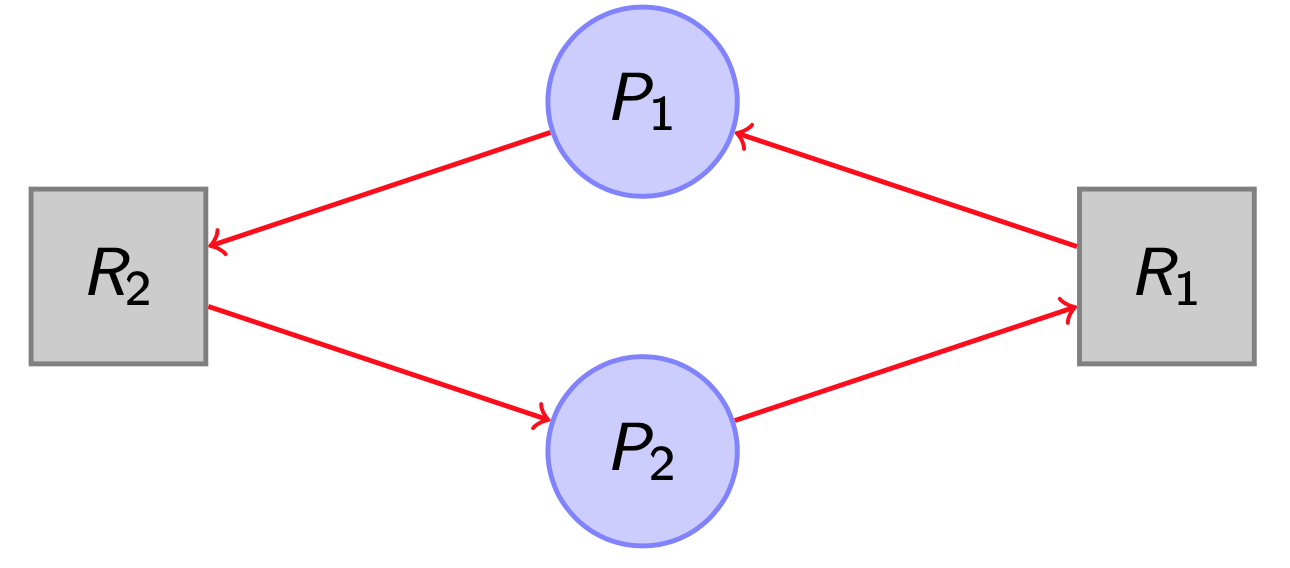
\includegraphics[width=0.6\textwidth]{imagenes/deadlock}

\subsubsection{Administración de E/S - ¿Por qué los algoritmos de scheduling se miden en cilindros? ¿Está bien? ¿Por qué? Explicar SAN}
Se llama \textit{seek time} al tiempo que tarda el brazo de un HDD en transportar los cabezales al cilindro correspondiente. El tiempo de accesso depende mayormente del \textit{seek time} y de la latencia de rotación.

Los algoritmos de scheduling de E/S definen de qué manera se moverá el brazo del disco lo cual determina el orden en que se atenderán los pedidos, en función del número de cilindro de cada uno. Cuanta más distancia recorra el brazo para cumplir los pedidos, mayor será el \textit{seek time} y más tardará en completarlos. Se miden en cilindros porque es la unidad de distancia del movimiento del brazo, cuanto mejor estén ordenados los pedidos, menos cilindros el brazo tendrá que recorrer para servirlos y mejor será el tiempo hasta completarlos.

SAN significa Storage Area Network. Se trata de tener el almacenamiento en la red, pero una red especial, donde los protocolos son específicos para este tipo de datos (son de más bajo nivel). 

El problema de tener Network Attached Storage (NAS) es que las operaciones consumen ancho de banda repercutiendo en la comunicación de la red.

\subsubsection{Seguridad - Explicar qué es una función de hash segura y ejemplificar dos usos en un sistema operativo. - comparar DAC y MAC}

Una función de hash segura es aquella que tiene muy baja probabilidad de generar colisiones y que sea muy difícil de revertir, es decir, sabiendo $y$ encontrar $x$ siendo $f(x) = y$, con $f$ la función de hash.

Discretionary Access Control (DAC): El acceso se controla basandose en las identidades de los usuarios y grupos. Se puede implementar con una matriz donde se almacena para cada sujeto, los distintos permisos sobre cada objeto. Los atributos de seguridad se definen explicitamente (se puede hacer solamente lo que está especificado). Es el usuario dueño del archivo quien determina quiénes tienen acceso al mismo.

Mandatory Access Control (MAC): Cada sujeto tiene un grado (se suele manejar el concepto de label). Los objetos heredan el grado/label del último sujeto que los modificó. Un sujeto sólo puede acceder a objetos de grado igual o menor que el suyo.

\subsubsection{Filesystems - Explicar journaling en ext3. ¿Qué problema resuelve?}

Cuando el sistema quiere realizar una transacción, en lugar de realizarla inmediatamente, se la escribe en el \textit{journal}. A esto se lo llama realizar un \textit{commit}. Un vez hecho el \textit{commit}, se devuelve el control al proceso usuario mientras el filesystem hace el replay de los commits registrados.

Este otro proceso mantiene un puntero que indica la operación dentro del commit que se está llevando a cabo, el cual va moviendo a medida que va satisfaciendo las operaciones y con ellas, los commits. Este algoritmo permite que ante una falla completa del sistema que requiera un reinicio, se pueda consultar el \textit{journal} para asi reestablecer el sistema mediante el puntero, y continuar con la operación que habia quedado pendiente, asi como con el resto de los commits que aún no habían sido ejecutados.